% Here you must respond to what the results mean. Probably it is the easiest section to write, but the hardest section to get right. This is because it is the most important section of your article. Here you get the chance to sell your data. Take into account that a huge numbers of manuscripts are rejected because the Discussion is weak.

% You need to make the Discussion corresponding to the Results, but do not reiterate the results. Here you need to compare the published results by your colleagues with yours (using some of the references included in the Introduction). Never ignore work in disagreement with yours, in turn, you must confront it and convince the reader that you are correct or better.

% Take into account the following tips:

% \begin{enumerate}
% \item  Avoid statements that go beyond what the results can support.
% \item Avoid unspecific expressions such as "higher temperature", "at a lower rate", "highly significant". Quantitative descriptions are always preferred.
% \item Avoid sudden introduction of new terms or ideas; you must present everything in the introduction, to be confronted with your results here.
% \item  Speculations on possible interpretations are allowed, but these should be rooted in fact, rather than imagination. To achieve good interpretations think about:  How do these results relate to the original question or objectives outlined in the Introduction section?
%     Do the data support your hypothesis?
%     Are your results consistent with what other investigators have reported?
%     Discuss weaknesses and discrepancies. If your results were unexpected, try to explain why
%     Is there another way to interpret your results?
%     What further research would be necessary to answer the questions raised by your results?
%     Explain what is new without exaggerating
% \item  Revision of Results and Discussion is not just paper work. You may do further experiments, derivations, or simulations. Sometimes you cannot clarify your idea in words because some critical items have not been studied substantially
% \end{enumerate}


% \subsection{Validation Methodology}\label{sec:results:validation}
% 




In \cite{Verendel_2009} Verendel finds 4 distinct validation methods used across the 90 security metrics papers surveyed: hypothetical, empirical, simulation, and theoretical. The author adds the caveat that no attempt was made to verify the quality of results, only to describe the methods used in each paper to substantiate the findings. In this section we propose a method for validating security metrics through empirical means.

In general, a metric should be both reliable and valid, where reliability refers to the consistency of values across repeated measurements, and validity concerns the accuracy of those values. There is currently no \textit{unit} reference for a security property which we can use for establishing the accuracy of our security metrics. We can, however, examine the behaviour of a metric relative to a given system by manipulating relevant aspects of that system while holding the other properties constant. For example, we can assign vulnerabilities to the small enterprise network shown in Figure \ref{fig:refnet_small}. For metrics that are influenced by the vulnerability score (such as CVSS based metrics), we can fix the weights of these vulnerabilities in the range of possible scores (0.0 to 10.0 in the case of CVSS). This would produce the lower and upper bound for that metric on this specific configuration of system configuration and vulnerability assignment. Similarly, we can alter properties such as the effects of a successful exploit (remote code execution, privilege escalation, etc), the placement and quantity of vulnerabilities, the underlying platform/operating system/applications, connectivity and topology, and so on. By capturing the measured values of controlled alterations to a system, we begin to understand how that metric behaves on the given system. Observing how multiple metrics behave under the same alterations allows us to compare their relative performance without an absolute point of reference. Furthermore, we can extend this analysis from a simple enterprise network to any number of use cases by supplying input adaptors for topology generators such as BRITE\cite{Medina_Lakhina_Matta_Byers_2001} or simulators like SSFNet\cite{Cowie_Ogielski_Nicol_2002} and Mininet\cite{Lantz_Heller_McKeown_2010}. Figure \ref{fig:refnets} shows an example reference set of 3 network topologies of increasing size and complexity. The first represents the type of example network commonly referenced in the literature to demonstrate a newly proposed metric, and the other two were selected from the gallery of publicly available SSFNet topologies and are described by an easy to parse domain specific language. By including systems at different scales, we are able to determine if a metric's performance depends on the size and complexity of the system under test. Intuitively, we would expect the temperature of 1 liter of boiling water to be the same as 1000 liters of boiling water, so testing against systems of varying size allows us to verify this hypothesis.

\begin{figure*}
    \centering
    \begin{subfigure}[t]{0.3\textwidth}
        % \centering
        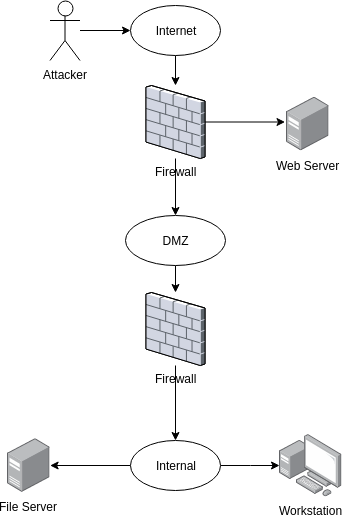
\includegraphics[width=\linewidth]{resource/img/ch_automation/from_ares_paper/net_small.png} 
        \caption{Small-sized network\cite{Ou_Appel_2005}} 
        \label{fig:refnet_small}
    \end{subfigure}
          \begin{subfigure}[t]{0.33\textwidth}
        \centering
        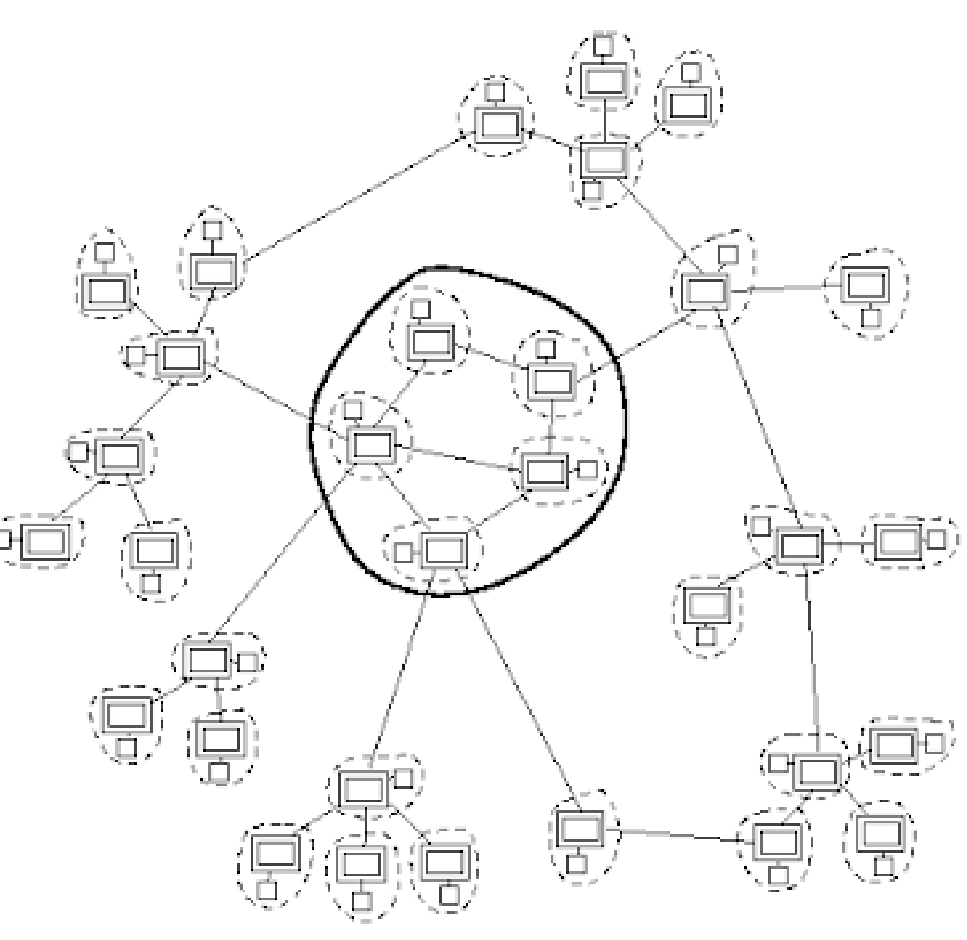
\includegraphics[width=\linewidth]{resource/img/ch_automation/from_ares_paper/net_med_2.png}
        \caption{Medium-sized network\cite{Cowie_Ogielski_Nicol_2002}}
        \label{fig:refnet_med}
    \end{subfigure}
     \begin{subfigure}[t]{0.3\textwidth}
        \centering
        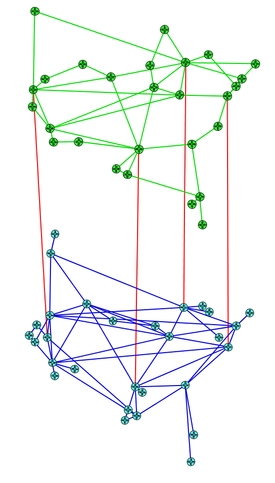
\includegraphics[width=\linewidth]{resource/img/ch_automation/from_ares_paper/net_large.png}
        \caption{Large-sized  network\cite{Cowie_Ogielski_Nicol_2002}}
        \label{fig:refnet_large}
    \end{subfigure}
    \hfill
    \caption{Different Sized Reference Networks}
    \label{fig:refnets}
\end{figure*}

If we consider a security metric as a measurement instrument, then we can validate the metric by characterizing its behavior against a reference set. Some security metric properties we might consider for validation can be taken directly from the field of measurement theory. In addition to accuracy and precision, Morris\cite{Morris_2001} describes several performance characteristics of measurement instruments that we may adapt to our validation of security metrics:

\textbf{Monotonicity}: Does the measured value always increase or always decrease with respect to each improvement in security.

\textbf{Linearity}: For security levels $s_1$ and $s_2$ and incremental security improvement $i$, is the difference between $(s_1,i)$ the same as $(s_2,i)$?

\textbf{Range}: What are the upper and lower bounds that a metric will assume for a specific model?

\textbf{Precision}: Does the metric report the same value for repeated measurements of the same quantity? This is of particular interest in probabilistic metrics. 

Analogues to other standard instrument performance measures - threshold, resolution, sensitivity to disturbance, etc - can be adapted to evaluate a security metric against our reference networks as well, and it is still to be determined which characteristics of static measurement instruments are required for their security related counterparts. 



% \subsection{Security Metrics as a Service}\label{sec:results:smaas}
% \input{content/results/smaas.tex}


In the security metrics surveys we reviewed in Section \ref{sec:litreview} there were over 500 distinct security metrics identified. The surveys each provided their own classification systems which were appropriate for the analysis they conducted, but none of these taxonomies generalize well to classify all types of security metrics. We describe properties common to all metrics, identify overlaps in the various taxonomies, identify points of confusion between existing metric hierarchies, and describe a suitable and intuitive system for classifying any current or future security metric. In using the CyBOK as the underlying classification system we are also able to determine the distribution of metrics in each topic and identify areas of limited coverage which would benefit from future research. 

In reproducing the results from the literature, we faced several issues during implementation, particularly with model based security metrics. Often assumptions were made about the intermediate processing of the pipeline that weren't surfaced in the supporting examples of the publication. We note that many of the survey authors describe security metric validation as an area of concern in security metric research. In response to these concerns and to move forward in our own research, we identified a generalized four step processing pipeline that separates the core steps of this process. By following this workflow we have identified and implemented many reusable preprocessing components, allowing us to rapidly add new security metrics from the literature and immediately test the performance of those metrics against a growing number of input models we use as our reference set. 

By enforcing the 4 stage pipeline abstraction, we achieve several benefits. Each phase is modular so that replacing any piece in the pipeline is straight forward. By plugging in the static reference set to the input phase we create a \textit{unit test} of sorts for our metric library, SecMet. With PTaH, the preprocessing and transformation handlers described above, we can articulate how any or all of the security metrics will behave under a variety of conditions for any given input - not just the reference set we describe above. This, in theory at least, should make characterizing the behaviours of security metrics on internal or sensitive systems as simple as adding input adapters to the existing set, which already includes Nessus, OVAL, NVD, CVE, and now SSFNet. By replacing our validation PTaH with whatever workflow execution engine is already in place, Apache Beam or Storm for example, the SecMet catalog becomes a drop in security measurement aid to support SecDevOps which we refer to as Security Metrics as a Service (S-MaaS).

Our takeaways from the experiments described above indicate that, while validating security metrics is not done rigorously in many of the publications, a mechanism for validation and analysis is not out of reach. By streamlining the development and evaluation process with automation, we aim to lower the barrier to entry in the field and allow researchers to spend more time developing and analyzing security metrics, which in turn should encourage more secure systems being deployed. 



